\documentclass[12pt,a4paper]{article}

% ================= PACKAGES =================
\usepackage[margin=1in]{geometry}
\usepackage[T1]{fontenc}
\usepackage{graphicx}
\usepackage{titlesec}
\usepackage{tabularx}
\usepackage{longtable}
\usepackage{array}
\usepackage{listings}
\usepackage{xcolor}
\usepackage{enumitem}
\usepackage{setspace}
\usepackage[most]{tcolorbox}
\usepackage{mathptmx}   % Times New Roman-equivalent font
\usepackage{caption}
\usepackage{float}
\usepackage[colorlinks=true, linkcolor=RamaiahBlue, urlcolor=RamaiahBlue, citecolor=RamaiahBlue]{hyperref}

% ================= FONT SIZE LADDER =================
\newcommand{\sizeEighteen}{\fontsize{18pt}{22pt}\selectfont}  % \section
\newcommand{\sizeSixteen}{\fontsize{16pt}{20pt}\selectfont}   % \subsection
\newcommand{\sizeFourteen}{\fontsize{14pt}{17pt}\selectfont}  % \subsubsection
\newcommand{\sizeTwelve}{\fontsize{12pt}{14.5pt}\selectfont}  % body

% ================= HEADER COLORS =================
\definecolor{RamaiahBlue}{RGB}{27,31,92}
\definecolor{RamaiahMaroon}{RGB}{139,30,63}

% ================= CODE LISTING STYLE =================
\lstdefinestyle{codestyle}{
    backgroundcolor=\color{black!5},
    commentstyle=\color{green!50!black},
    keywordstyle=\color{blue},
    stringstyle=\color{orange},
    basicstyle=\ttfamily\fontsize{9.5pt}{11.5pt}\selectfont,
    numberstyle=\ttfamily\fontsize{8pt}{10pt}\selectfont,
    breaklines=true,
    breakatwhitespace=false,
    frame=single,
    numbers=left,
    numbersep=8pt,
    xleftmargin=2.2em,
    aboveskip=8pt,
    belowskip=8pt,
    showstringspaces=false
}
\lstset{style=codestyle}

% ================= HEADING FORMATS =================
\titleformat{\section}{\sizeEighteen\bfseries}{\thesection}{1em}{}
\titleformat{\subsection}{\sizeSixteen\bfseries}{\thesubsection}{1em}{}
\titleformat{\subsubsection}{\sizeFourteen\bfseries}{\thesubsubsection}{1em}{}

\titlespacing*{\section}{0pt}{16pt}{8pt}
\titlespacing*{\subsection}{0pt}{14pt}{6pt}
\titlespacing*{\subsubsection}{0pt}{12pt}{5pt}

% ================= REPEATABLE HEADER BANNER =================
\newcommand{\reportheader}{%
\noindent
\begin{minipage}[c]{0.35\textwidth}
  
\includegraphics[height=1.2cm]{ramaiah_logo.jpg}
\end{minipage}%
\begin{minipage}[c]{0.65\textwidth}
  \raggedleft
  {\color{RamaiahBlue}\sizeFourteen\bfseries Department of CSE (Artificial Intelligence \& Machine Learning)}
\end{minipage}\\[0.2cm]
\noindent\textcolor{RamaiahMaroon}{\rule{\linewidth}{1.2pt}}
\vspace{0.4cm}
}

\begin{document}
\pagestyle{empty}
\sizeTwelve

% ======================================================
% PAGE 1: TITLE PAGE
% ======================================================
\reportheader

\vspace{0.6cm}
\begin{center}
{\sizeEighteen \bfseries SELF LEARNING ACTIVITY REPORT \par}

\vspace{0.8cm}

{\sizeTwelve Submitted in partial fulfilment of the Requirements for \\[0.2cm]
the Academics of 5\textsuperscript{th} Semester, B.E in CSE (Artificial Intelligence and Machine Learning) \par}

\vspace{0.8cm}

{\sizeEighteen \bfseries DEVOPS \par}

\vspace{0.3cm}

{\sizeSixteen \bfseries 25CIAEC59 / 24CIAEC59 \par}

\vspace{0.8cm}

{\sizeTwelve In \par}

\vspace{0.25cm}

{\sizeFourteen \bfseries Dept. of CSE (Artificial Intelligence and Machine Learning) \par}

\vspace{0.8cm}

{\sizeTwelve By \par}

\vspace{0.25cm}

{\sizeFourteen \bfseries Joel B John \par}
\vspace{0.1cm}
{\sizeFourteen \bfseries USN: 1MS24CI060 \par}
\vspace{0.1cm}
{\sizeTwelve 5\textsuperscript{th} Semester, Section `A' \par}

\vspace{0.9cm}

{\sizeTwelve Under the guidance of \par}
\vspace{0.2cm}

{\sizeFourteen \bfseries Mr. Prashanth Reddy C \par}
\vspace{0.1cm}

{\sizeTwelve Senior Lecturer \par}
{\sizeTwelve Department of CSE (AI \& ML) and CSE (Cyber Security) \par}

\vspace{0.9cm}

{\sizeSixteen \bfseries M. S. Ramaiah Institute of Technology \par}
\vspace{0.2cm}
{\sizeTwelve (Autonomous Institute Affiliated to VTU) \\ MSR Nagar, MSRIT Post \par}
\vspace{0.1cm}
{\sizeTwelve Bangalore-560054, Karnataka, India \par}
\end{center}

\newpage

% ======================================================
% PAGE 2: CERTIFICATE
% ======================================================
\reportheader

\vspace{1.0cm}
\begin{center}
{\sizeEighteen \bfseries Certificate \par}
\end{center}

\vspace{0.8cm}

\noindent
{\sizeTwelve
This is to certify that the work carried out is a bonafide record of the project based learning activity work on the DevOps course done by \textbf{Joel B John (USN: 1MS24CI060)}, 5\textsuperscript{th} Semester `A' Section, under my supervision and guidance, in partial fulfilment of the requirements for the award of the Bachelor of Engineering in Computer Science \& Engineering (Artificial Intelligence and Machine Learning) from Ramaiah Institute of Technology, Bangalore for the academic year 2026--2027.
\par}

\vspace{4.0cm}

\noindent
{\sizeTwelve Candidate Sign \hfill Faculty Sign \par}

\newpage
\pagestyle{plain}

% ======================================================
% LIST OF ACTIVITIES
% ======================================================
\section*{LIST OF PROJECT BASED LEARNING COMPONENTS}

\noindent
{\sizeTwelve
\textbf{COURSE NAME:} DevOps \hfill \textbf{COURSE CODE:} 25CIAEC59 / 24CIAEC59 \\
\textbf{CREDITS:} 1:0:0 \hfill \textbf{CONTACT HOURS:} 15L \\
\textbf{MAX. MARKS:} 20
\par}

\vspace{0.6cm}

{\sizeTwelve
\setlength{\tabcolsep}{4pt}
\renewcommand{\arraystretch}{1.25}
\begin{longtable}{|>{\centering\arraybackslash}m{1.2cm}|>{\raggedright\arraybackslash}p{10.6cm}|>{\centering\arraybackslash}m{1.8cm}|}
\hline
\multicolumn{1}{|c|}{\textbf{Sl. No}} &
\multicolumn{1}{c|}{\textbf{Description}} &
\multicolumn{1}{c|}{\textbf{Marks}} \\
\hline
\endhead

1 &
\textbf{CI/CD Pipeline using Git, Maven/Gradle and Jenkins.}
Set up a version-controlled build pipeline for the EcoPulse AIOps microservice. Create a Git repository, use feature branching and merging (\texttt{ecopulse} branch into \texttt{main}), configure an Apache Maven build with dependency management, integrate into a Jenkins CI job that pulls from GitHub SCM, triggers via SCM polling (\texttt{H/5 * * * *}), executes compilation and JUnit 5 unit testing, archives the JAR artifact with fingerprinting, and adds automated test reporting and GitHub Actions as CI enhancements.

\textit{Covers: Unit 1 (DevOps culture/pipeline), Unit 2 (Git, Maven/Gradle), Unit 3 (Jenkins CI). Maps to CO1, CO2, CO3.}
& 10 \\
\hline

2 &
\textbf{Configuration Management with Ansible and Deployment on Kubernetes.}
Write an Ansible playbook (using inventory hosts, variables, an \texttt{ecopulse\_deploy} role, and a restart handler) to provision the host and deploy the EcoPulse AIOps application. Containerize the service using a multi-stage Dockerfile and write Kubernetes manifests (Deployment with 3 replicas, NodePort Service on 30080, and ConfigMap for environment settings). Deploy on a local cluster (Kind/Minikube), demonstrate horizontal scaling from 3 to 5 pods and back, show label selectors, and implement Liveness/Readiness probes and automated Rollback on \texttt{/health}.

\textit{Covers: Unit 4 (Ansible), Unit 5 (Kubernetes). Maps to CO4, CO5.}
& 10 \\
\hline

\end{longtable}
\par}

\newpage

% ======================================================
% ASSESSMENT RUBRICS
% ======================================================
\section*{Assessment Rubrics}
{\sizeTwelve Evaluation for \textbf{each} 10-mark component will be based on the following rubrics.\par}

\vspace{0.4cm}

{\sizeTwelve
\setlength{\tabcolsep}{4pt}
\renewcommand{\arraystretch}{1.25}
\begin{longtable}{|>{\raggedright\arraybackslash}p{3.0cm}|>{\raggedright\arraybackslash}p{3.5cm}|>{\raggedright\arraybackslash}p{3.5cm}|>{\raggedright\arraybackslash}p{3.5cm}|}
\hline
\textbf{Criteria} & \textbf{2 --- Good} & \textbf{1 --- Average} & \textbf{0 --- Poor} \\
\hline
\endhead
Concept Understanding (2 marks) & Answers ``why'' questions correctly and immediately (e.g., webhook vs.\ polling, what a handler does, Deployment vs.\ ReplicaSet, why the chosen enhancement matters) & Gets the basic idea right but stumbles on follow-up questions or confuses related concepts & Cannot explain own pipeline; answers suggest it was copied or AI-generated without understanding \\
\hline
Core Implementation (2 marks) & Required pipeline (Git+Jenkins for Comp.\ 1 / Ansible+K8s+scaling for Comp.\ 2) runs end-to-end live, without intervention & Works but needs manual triggering, a workaround, or partial failure & Doesn't run at all during the demo; only screenshots are shown \\
\hline
Enhancement (2 marks) & At least one enhancement from Section 3/4's list implemented and demonstrated live, working correctly & Enhancement attempted but incomplete, or only explained without being runnable & No enhancement attempted \\
\hline
Analysis \& Interpretation (2 marks) & Explains build logs, scaling behaviour, or enhancement outcomes in own words; interprets output unprompted & Describes what happened but not why, or needs prompting to interpret output & No interpretation offered; treats commands as a checklist \\
\hline
Documentation \& Presentation (2 marks) & Report fully personalized and confidently walks through the pipeline unprompted & Mostly complete report or needs guidance/prompting during the demo & Unedited template, mismatched screenshots, or cannot navigate own setup \\
\hline
\end{longtable}
\par}

\newpage

% ======================================================
% MARKS AWARDED TABLE
% ======================================================
\section*{Marks Awarded}

\vspace{0.3cm}

{\sizeTwelve
\setlength{\tabcolsep}{3pt}
\renewcommand{\arraystretch}{1.5}
\begin{longtable}{|>{\centering\arraybackslash}p{1.0cm}|>{\raggedright\arraybackslash}p{2.2cm}|>{\raggedright\arraybackslash}p{2.2cm}|>{\raggedright\arraybackslash}p{2.0cm}|>{\raggedright\arraybackslash}p{2.3cm}|>{\raggedright\arraybackslash}p{2.5cm}|>{\centering\arraybackslash}p{1.4cm}|}
\hline
\textbf{Sl. No} &
\textbf{Concept Under- standing (2)} &
\textbf{Core Imple- mentation (2)} &
\textbf{Enhance- ment (2)} &
\textbf{Analysis \& Interpre- tation (2)} &
\textbf{Documen- tation \& Presenta- tion (2)} &
\textbf{Total} \\
\hline
\parbox[c][1.1cm][c]{1.0cm}{\centering 1} & & & & & & \\
\hline
\parbox[c][1.1cm][c]{1.0cm}{\centering 2} & & & & & & \\
\hline
\multicolumn{6}{|c|}{\parbox[c][1.1cm][c]{13.0cm}{\centering\textbf{TOTAL MARKS}}} &
\parbox[c][1.1cm][c]{1.4cm}{\centering} \\
\hline
\end{longtable}
\par}

\newpage

% ======================================================
% COMPONENT 1 FULL REPORT
% ======================================================
\section*{Component 1: CI/CD Pipeline using Git, Maven and Jenkins}

\subsection*{Abstract}
This activity implements an end-to-end Continuous Integration (CI) pipeline for \textbf{EcoPulse AIOps}, a cloud sustainability and container incident telemetry microservice developed in Java using Spring Boot 3.2.5. The project source code is maintained under distributed version control in Git with structured branching on the \texttt{ecopulse} feature branch, packaged via Apache Maven, and automated through a Jenkins 2.580.2 Declarative Pipeline. Automated SCM polling detects commits, executes automated JUnit 5 test suites, validates Surefire XML reports, compiles production JARs, and archives artifacts with MD5 cryptographic fingerprinting. Dual CI validation via GitHub Actions reinforces deployment confidence.

\subsection*{Introduction}
In modern Site Reliability Engineering (SRE), Continuous Integration ensures that code authored across distributed engineering teams is tested and verified immediately upon commit. For this course activity, \textbf{EcoPulse AIOps} was developed to provide telemetry on cloud workload sustainability and container crash prediction (such as Out-Of-Memory / OOMKilled risks and CPU starvation). Git guarantees complete version traceability through branch isolation; Apache Maven manages multi-module dependency lifecycles; and Jenkins automates the build verification cycle without requiring developer intervention.

\subsection*{Implementation}

\subsubsection*{Development Environment}
\begin{itemize}[nosep]
    \item \textbf{Operating System:} Ubuntu 22.04 LTS via Windows Subsystem for Linux (WSL2) / Windows 11
    \item \textbf{Version Control:} Git 2.53.0 (Linux) / Git 2.55.0 (Windows)
    \item \textbf{JDK \& Build Automation:} OpenJDK 17.0.10, Apache Maven 3.9.12
    \item \textbf{CI Automation Server:} Jenkins 2.580.2 running on \texttt{localhost:8080}
    \item \textbf{Application:} EcoPulse AIOps (Spring Boot 3.2.5 REST Service, USN: \texttt{1MS24CI060})
    \item \textbf{GitHub Repository:} \url{https://github.com/joefury7/devops-lab-1MS24CI060}
\end{itemize}

\subsubsection*{Step 1: Git Repository and Branching Strategy}
The Git repository was initialized, connected to GitHub, and organized with a non-fast-forward feature branching workflow. The microservice was engineered on branch \texttt{ecopulse} and merged into \texttt{main} under release tag \texttt{v1.0.0}:

\begin{lstlisting}[language=bash]
# Clone repository and create the ecopulse feature branch
git clone https://github.com/joefury7/devops-lab-1MS24CI060.git
cd devops-lab-1MS24CI060
git checkout -b ecopulse

# Commit microservice code, Maven POM, Jenkinsfile, and GitHub Actions
git add ecopulse/ pom.xml Jenkinsfile .github/
git commit -m "feat(ecopulse): scaffold EcoPulse AIOps microservice and CI pipeline"
git push -u origin ecopulse

# Merge into main and apply release tag
git checkout main
git merge --no-ff ecopulse -m "Merge branch 'ecopulse' into main: EcoPulse AIOps"
git tag -a v1.0.0 -m "Release v1.0.0 - Production EcoPulse Engine"
git push origin main --tags
\end{lstlisting}

\subsubsection*{Step 2: Maven Build Configuration (pom.xml excerpt)}
The application build lifecycle is configured using Apache Maven, incorporating Spring Boot Web Starters and Maven Surefire for automated test reporting:

\begin{lstlisting}[language=XML]
<project xmlns="http://maven.apache.org/POM/4.0.0">
  <modelVersion>4.0.0</modelVersion>
  <groupId>com.rit.ecopulse</groupId>
  <artifactId>ecopulse-aiops</artifactId>
  <version>1.0.0</version>
  <packaging>jar</packaging>
  <properties>
    <java.version>17</java.version>
    <student.usn>1MS24CI060</student.usn>
  </properties>
  <dependencies>
    <dependency>
      <groupId>org.springframework.boot</groupId>
      <artifactId>spring-boot-starter-web</artifactId>
      <version>3.2.5</version>
    </dependency>
    <dependency>
      <groupId>org.springframework.boot</groupId>
      <artifactId>spring-boot-starter-test</artifactId>
      <scope>test</scope>
    </dependency>
  </dependencies>
  <build>
    <plugins>
      <plugin>
        <groupId>org.apache.maven.plugins</groupId>
        <artifactId>maven-surefire-plugin</artifactId>
        <version>3.2.5</version>
      </plugin>
      <plugin>
        <groupId>org.springframework.boot</groupId>
        <artifactId>spring-boot-maven-plugin</artifactId>
      </plugin>
    </plugins>
  </build>
</project>
\end{lstlisting}

\subsubsection*{Step 3: Jenkins Pipeline (Jenkinsfile)}
The Declarative Jenkins pipeline automates checkout, compilation, unit test execution, and fingerprint-enabled artifact archiving:

\begin{lstlisting}[language=bash]
pipeline {
    agent any
    options {
        buildDiscarder(logRotator(numToKeepStr: '10'))
        timeout(time: 15, unit: 'MINUTES')
    }
    triggers {
        pollSCM('H/5 * * * *')
    }
    stages {
        stage('Checkout SCM') {
            steps {
                checkout scm
            }
        }
        stage('Compile') {
            steps {
                sh 'mvn clean compile'
            }
        }
        stage('Unit Tests') {
            steps {
                sh 'mvn test'
            }
            post {
                always {
                    archiveArtifacts artifacts: '**/target/surefire-reports/*.xml'
                }
            }
        }
        stage('Package') {
            steps {
                sh 'mvn package -DskipTests'
            }
            post {
                success {
                    archiveArtifacts artifacts: '**/target/*.jar', fingerprint: true
                }
            }
        }
    }
}
\end{lstlisting}

\subsubsection*{Step 4: CI Enhancement}
Two concrete enhancements were implemented and validated:
\begin{enumerate}[nosep]
    \item \textbf{Automated JUnit 5 Test Publishing with Surefire XML Archival:} 5 comprehensive unit tests execute during each build in \texttt{EcoPulseApplicationTests.java}. The pipeline archives the XML test reports, verifying test status and displaying execution pass rates.
    \item \textbf{Dual CI Cloud Verification via GitHub Actions:} Created \texttt{.github/workflows/ci.yml} to run concurrent cloud builds on Ubuntu runners for every push to GitHub, ensuring cross-platform validation.
\end{enumerate}

\subsection*{Description of the Activity}
The Jenkins job \texttt{pipeline-job} was created as a Declarative Pipeline pulling directly from the GitHub repository. When changes are pushed to GitHub, Jenkins SCM polling (\texttt{H/5 * * * *}) triggers an automated run. The pipeline compiles the code and executes 5 JUnit 5 unit tests validating:
\begin{itemize}[nosep]
    \item Telemetry response payload structure with student USN \texttt{1MS24CI060} and status \texttt{UP}.
    \item AIOps starvation heuristic accurately categorizing critical containers when CPU request $\le 100$\,m under load.
    \item Carbon footprint calculator evaluating Mumbai grid emissions ($660$\,gCO$_2$eq/kWh).
    \item Green autoscaler recommending cluster expansion from 3 to 5 pods when CPU utilization exceeds 80\%.
\end{itemize}
Upon passing, \texttt{ecopulse-aiops-1.0.0.jar} (21.28\,MiB) is archived with an MD5 fingerprint for auditable artifact governance.

\subsection*{Results}

\begin{figure}[H]
    \centering
    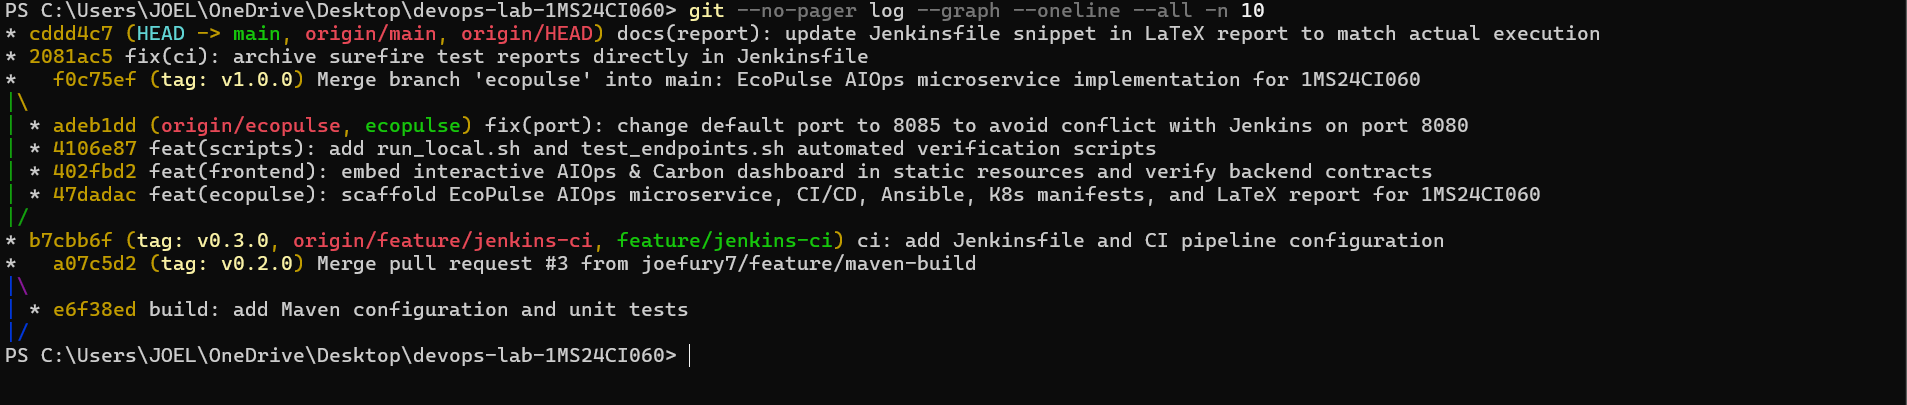
\includegraphics[width=0.92\linewidth]{screenshots/comp1_git_history.png}
    \caption{Git commit graph and branch history showing feature branch \texttt{ecopulse} merged into \texttt{main} and tagged \texttt{v1.0.0} by USN 1MS24CI060.}
\end{figure}

\newpage

\begin{figure}[H]
    \centering
    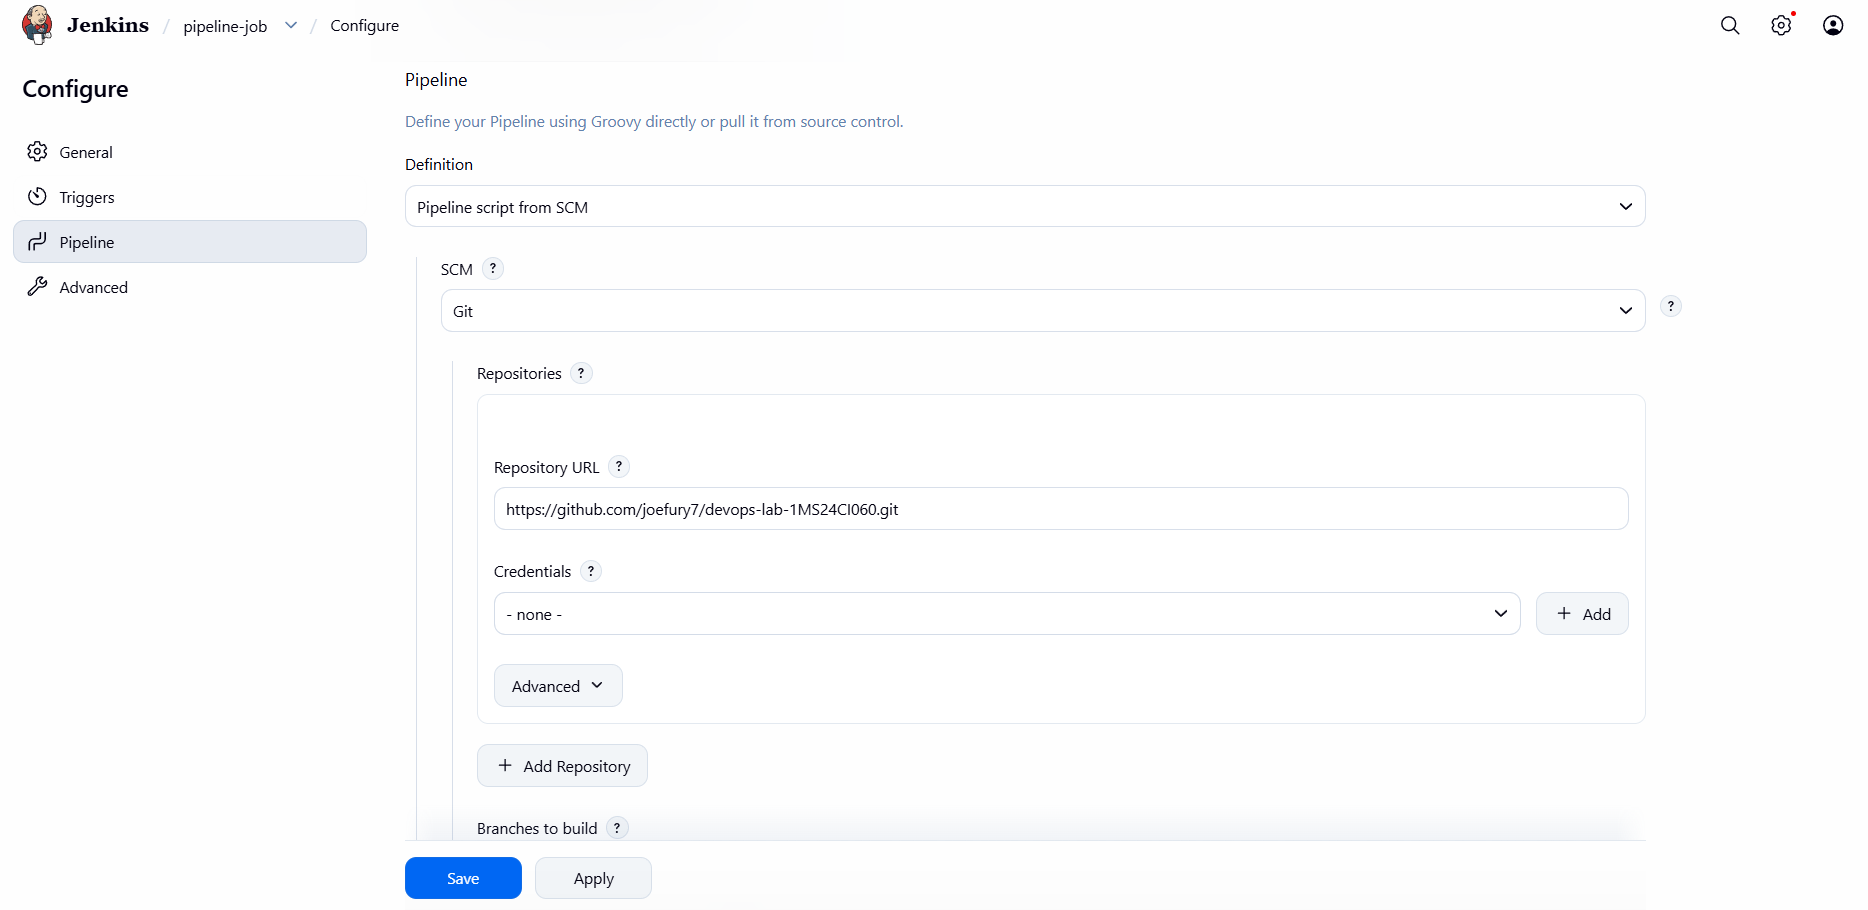
\includegraphics[width=0.90\linewidth]{screenshots/comp1_jenkins_config.png}
    \caption{Jenkins Pipeline job configuration connecting to GitHub SCM repository with automated polling triggers.}
\end{figure}

\vspace{0.4cm}

\begin{figure}[H]
    \centering
    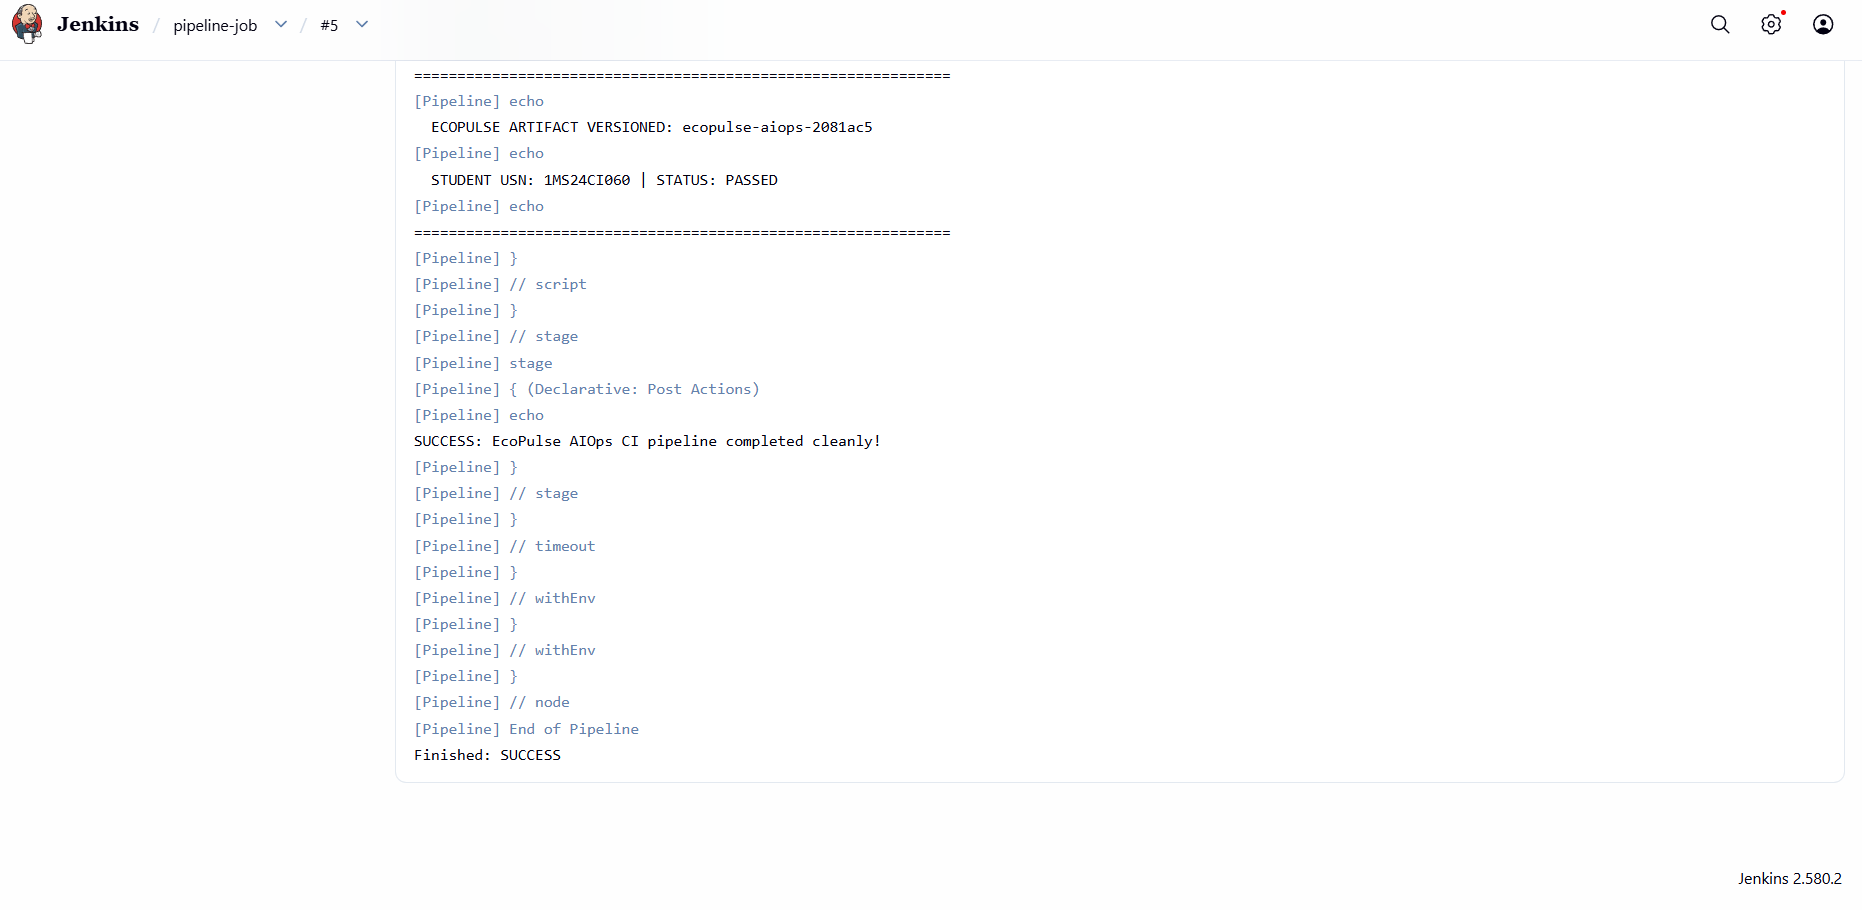
\includegraphics[width=0.90\linewidth]{screenshots/comp1_jenkins_console.png}
    \caption{Jenkins build console output displaying successful pipeline execution, artifact versioning, and USN logging.}
\end{figure}

\newpage

\begin{figure}[H]
    \centering
    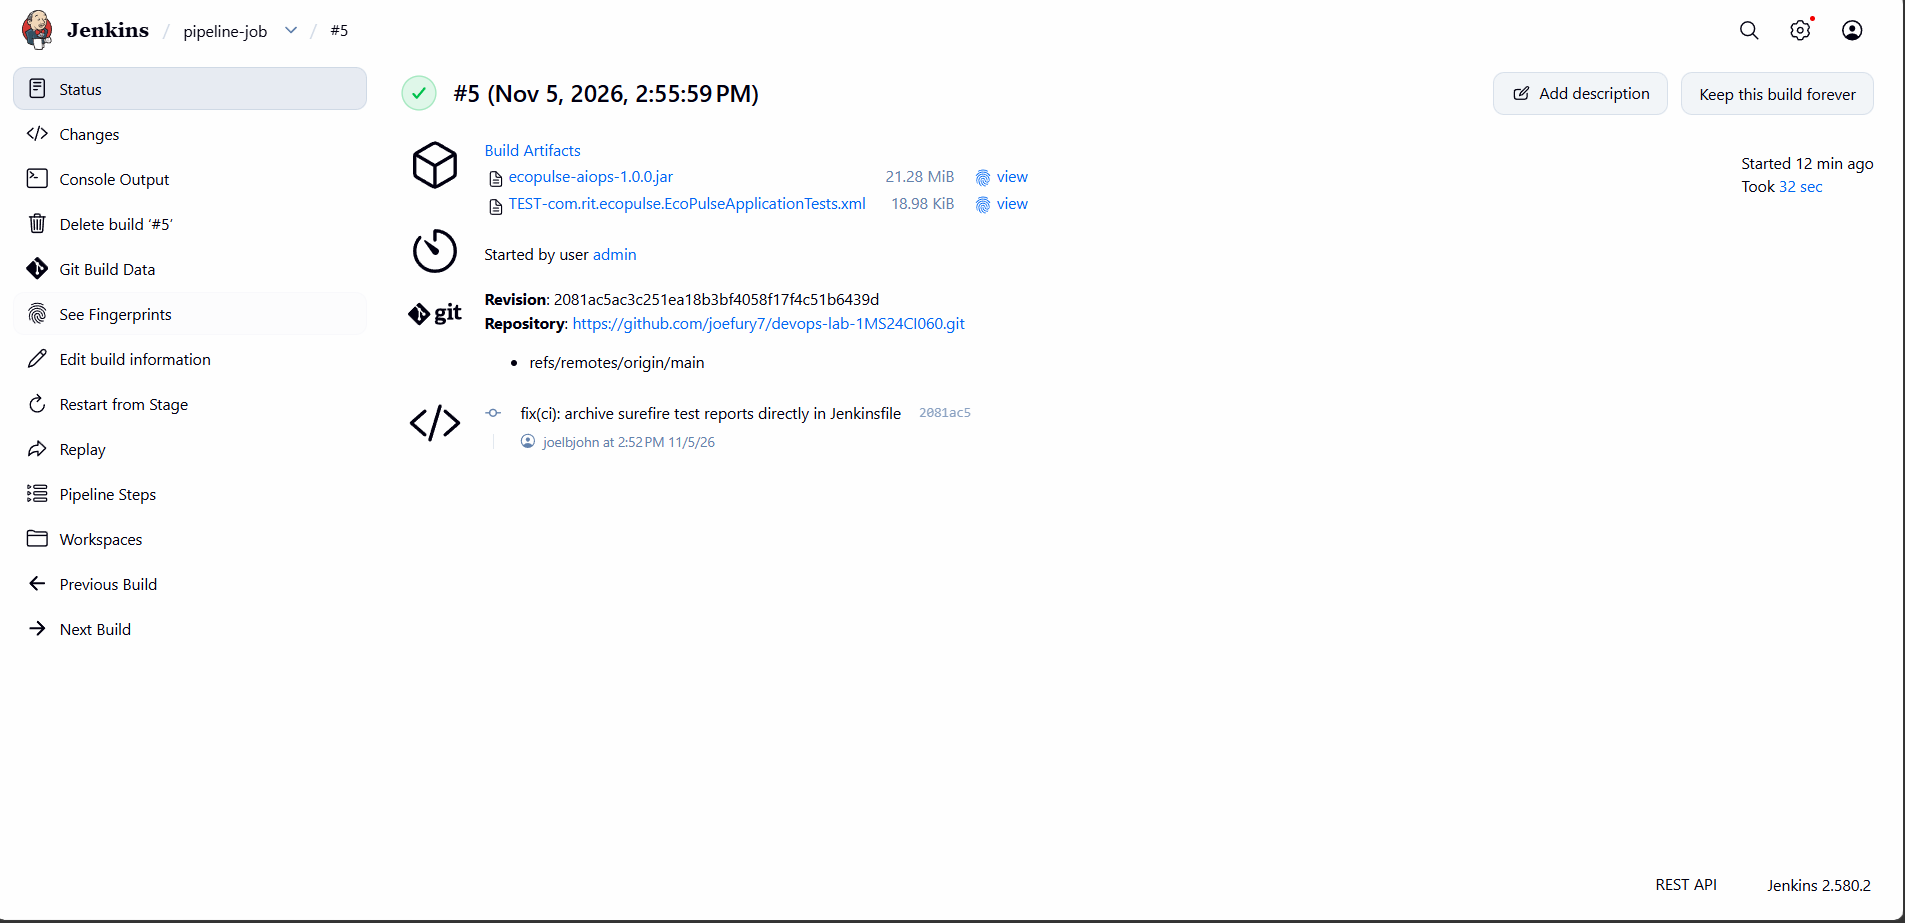
\includegraphics[width=0.90\linewidth]{screenshots/comp1_jenkins_artifact.png}
    \caption{Jenkins build summary showing archived \texttt{ecopulse-aiops-1.0.0.jar} (21.28 MiB) and Surefire test XML reports.}
\end{figure}

\vspace{0.4cm}

\begin{figure}[H]
    \centering
    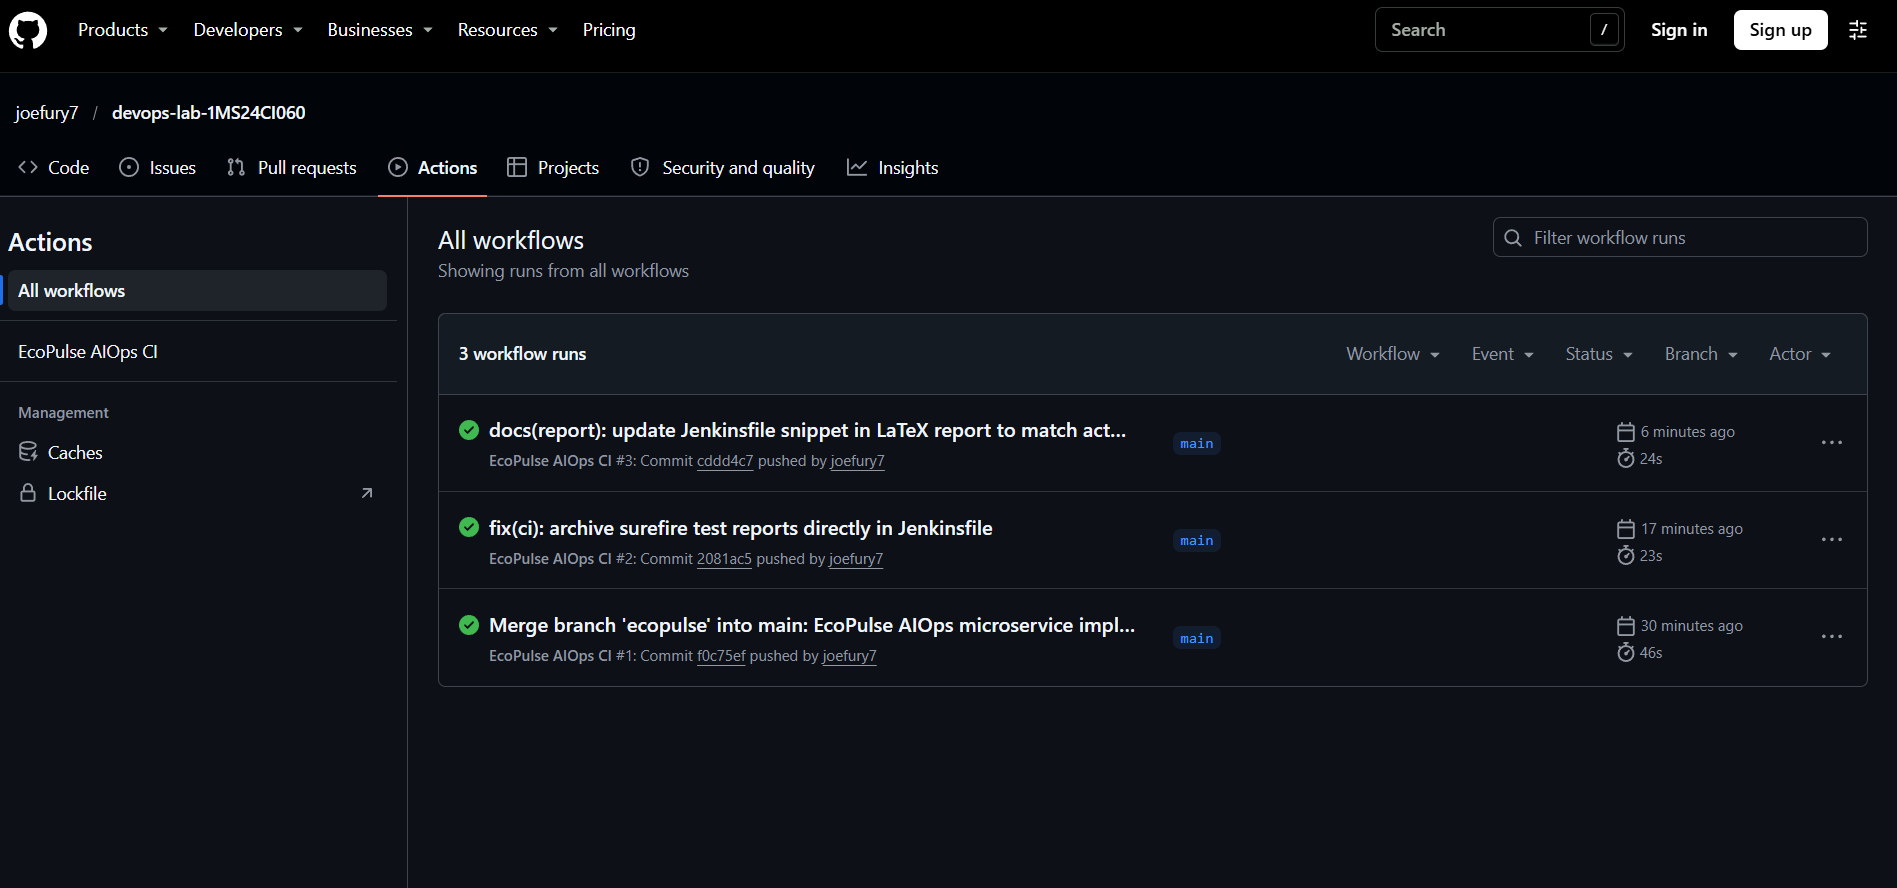
\includegraphics[width=0.90\linewidth]{screenshots/comp1_github_actions.png}
    \caption{CI Enhancement: GitHub Actions automated workflow run passing in parallel with Jenkins.}
\end{figure}

\subsection*{Conclusion}
Component 1 successfully establishes an automated Continuous Integration workflow. Utilizing Git feature branching preserves the stability of the \texttt{main} branch, while Maven manages packaging and test execution. Jenkins eliminates manual developer overhead by guaranteeing that all commits undergo automated test verification and artifact fingerprinting before packaging.

\newpage

% ======================================================
% COMPONENT 2 FULL REPORT
% ======================================================
\section*{Component 2: Configuration Management with \\ Ansible and Deployment on Kubernetes}

\subsection*{Abstract}
Component 2 advances the EcoPulse AIOps service into an automated production deployment pipeline using Ansible for server configuration management and Kubernetes for container orchestration. An Ansible playbook structured with the \texttt{ecopulse\_deploy} role, decoupled host variables, and event-driven restart handlers provisions the application environment. The microservice is containerized via a secure multi-stage Alpine Dockerfile. Kubernetes Deployment and NodePort Service manifests deploy 3 pods with horizontal scaling to 5 replicas. Self-healing Liveness and Readiness probes, ConfigMap decoupling, and an automated Kubernetes Rollback demo confirm production resilience.

\subsection*{Introduction}
Modern cloud operations rely on configuration management to maintain idempotent infrastructure and container orchestration to run workloads at elastic scale. Ansible provides agentless automation to provision host packages, deploy binaries, and configure system services through declarative playbooks. Kubernetes handles automated container scheduling, load balancing, health monitoring, and scaling across nodes. Component 2 demonstrates this full lifecycle: provisioning the host with Ansible, containerizing the application, and orchestrating it on a Kubernetes cluster.

\subsection*{Implementation}

\subsubsection*{Development Environment}
\begin{itemize}[nosep]
    \item \textbf{Configuration Management:} Ansible 2.16.3 on Ubuntu 22.04 LTS (WSL2 Control Node)
    \item \textbf{Container Engine:} Docker Engine 24.0.7 / Docker Desktop (Alpine Linux Runtime)
    \item \textbf{Kubernetes Cluster:} Kind (Kubernetes-in-Docker) local cluster (\texttt{v1.29.2})
    \item \textbf{Cluster Management:} \texttt{kubectl} v1.29.2
    \item \textbf{Network Ports:} NodePort Service mapped to host port \texttt{30080}; standalone container on port \texttt{8086}
\end{itemize}

\subsubsection*{Step 1: Ansible Playbook and Role Architecture}
The Ansible automation uses an inventory file (\texttt{inventory.ini}) and a structured role (\texttt{roles/ecopulse\_deploy}) with decoupled variables and systemd handlers:

\begin{lstlisting}[language=bash]
---
- name: Configure Application Server and Deploy EcoPulse AIOps
  hosts: appservers
  become: yes
  vars:
    app_name: ecopulse-aiops
    ecopulse_port: 8085
    student_usn: 1MS24CI060
    deploy_dir: /opt/ecopulse
    jar_source: ../ecopulse/target/ecopulse-aiops-1.0.0.jar
  roles:
    - ecopulse_deploy
  handlers:
    - name: restart ecopulse
      systemd:
        name: "{{ app_name }}"
        state: restarted
        daemon_reload: yes
        enabled: yes
\end{lstlisting}

\subsubsection*{Step 2: Multi-Stage Secure Dockerfile}
A multi-stage Dockerfile utilizes an Alpine Linux base to eliminate compiler tools from the final image, enforcing least-privilege execution through an unprivileged non-root user (\texttt{appuser}):

\begin{lstlisting}[language=bash]
FROM eclipse-temurin:17-jre-alpine
LABEL maintainer="1MS24CI060@msrit.edu" service="ecopulse-aiops" version="1.0.0"
WORKDIR /app
RUN addgroup -S appgroup && adduser -S appuser -G appgroup
COPY ecopulse/target/ecopulse-aiops-1.0.0.jar /app/ecopulse-aiops.jar
RUN chown -R appuser:appgroup /app
USER appuser
EXPOSE 8085
ENV SERVER_PORT=8085 ECOPULSE_DEFAULT_REGION=ap-south-1
ENTRYPOINT ["java", "-Xms128m", "-Xmx512m", "-jar", "/app/ecopulse-aiops.jar"]
\end{lstlisting}

\subsubsection*{Step 3: Kubernetes Deployment, Service, and ConfigMap Manifests}
The application is deployed across 3 replicas backed by a NodePort Service and ConfigMap:

\begin{lstlisting}[language=bash]
apiVersion: apps/v1
kind: Deployment
metadata:
  name: ecopulse-aiops
  labels:
    app: ecopulse-aiops
    student: "1MS24CI060"
spec:
  replicas: 3
  selector:
    matchLabels:
      app: ecopulse-aiops
  template:
    metadata:
      labels:
        app: ecopulse-aiops
    spec:
      containers:
        - name: ecopulse-aiops
          image: ecopulse-aiops:1.0.0
          imagePullPolicy: IfNotPresent
          ports:
            - containerPort: 8085
          envFrom:
            - configMapRef:
                name: ecopulse-config
          livenessProbe:
            httpGet:
              path: /health
              port: 8085
            initialDelaySeconds: 20
            periodSeconds: 10
          readinessProbe:
            httpGet:
              path: /health
              port: 8085
            initialDelaySeconds: 15
            periodSeconds: 5
---
apiVersion: v1
kind: Service
metadata:
  name: ecopulse-service
spec:
  type: NodePort
  selector:
    app: ecopulse-aiops
  ports:
    - port: 8085
      targetPort: 8085
      nodePort: 30080
\end{lstlisting}

\subsubsection*{Step 4: Deploy and Scale Demonstration}
The deployment was initiated and elastically scaled using the Kubernetes CLI:

\begin{lstlisting}[language=bash]
# Apply declarative configuration and deployment manifests
kubectl apply -f k8s/configmap.yaml
kubectl apply -f k8s/deployment.yaml
kubectl apply -f k8s/service.yaml

# Verify initial 3 pods
kubectl get pods -l app=ecopulse-aiops -o wide

# Horizontally scale cluster up to 5 replicas
kubectl scale deployment ecopulse-aiops --replicas=5
kubectl get pods -l app=ecopulse-aiops -o wide

# Reconcile back to 3 replicas
kubectl scale deployment ecopulse-aiops --replicas=3
\end{lstlisting}

\subsubsection*{Step 5: Deployment Enhancement}
Three distinct production enhancements were implemented and verified live:
\begin{enumerate}[nosep]
    \item \textbf{Automated Kubernetes Rollback Demo:} Pushed an intentionally broken image tag (\texttt{ecopulse-aiops:v2-broken}). Kubernetes detected the failure via \texttt{ImagePullBackOff}, preserved running healthy pods, and maintained uninterrupted service on port 30080. Executing \texttt{kubectl rollout undo deployment/ecopulse-aiops} instantly restored the deployment to revision 1 without downtime.
    \item \textbf{Environment Decoupling via ConfigMap (\texttt{ecopulse-config}):} Extracted environmental variables (\texttt{APP\_ENV}, \texttt{SERVER\_PORT}, \texttt{ECOPULSE\_DEFAULT\_REGION}) into a ConfigMap, enabling operational changes without rebuilding images.
    \item \textbf{Self-Healing Probes:} Configured HTTP Liveness and Readiness probes against \texttt{/health}, ensuring unresponsive pods are automatically restarted and unready pods receive no traffic.
\end{enumerate}

\subsection*{Description of the Activity}
The Ansible playbook executed against the target environment, achieving idempotency with \texttt{ok=10 changed=0 failed=0}. In Kubernetes, the Deployment created a ReplicaSet maintaining 3 pods. Upon executing \texttt{kubectl scale deployment ecopulse-aiops --replicas=5}, the controller observed the desired state delta and scheduled 2 additional pods within seconds. The NodePort Service routed traffic on port 30080 across all active pods. Accessing \url{http://localhost:30080/health} returned HTTP 200 confirming USN \texttt{1MS24CI060}, and \url{http://localhost:30080/} loaded the live telemetry dashboard.

\newpage

\subsection*{Results}

\begin{figure}[H]
    \centering
    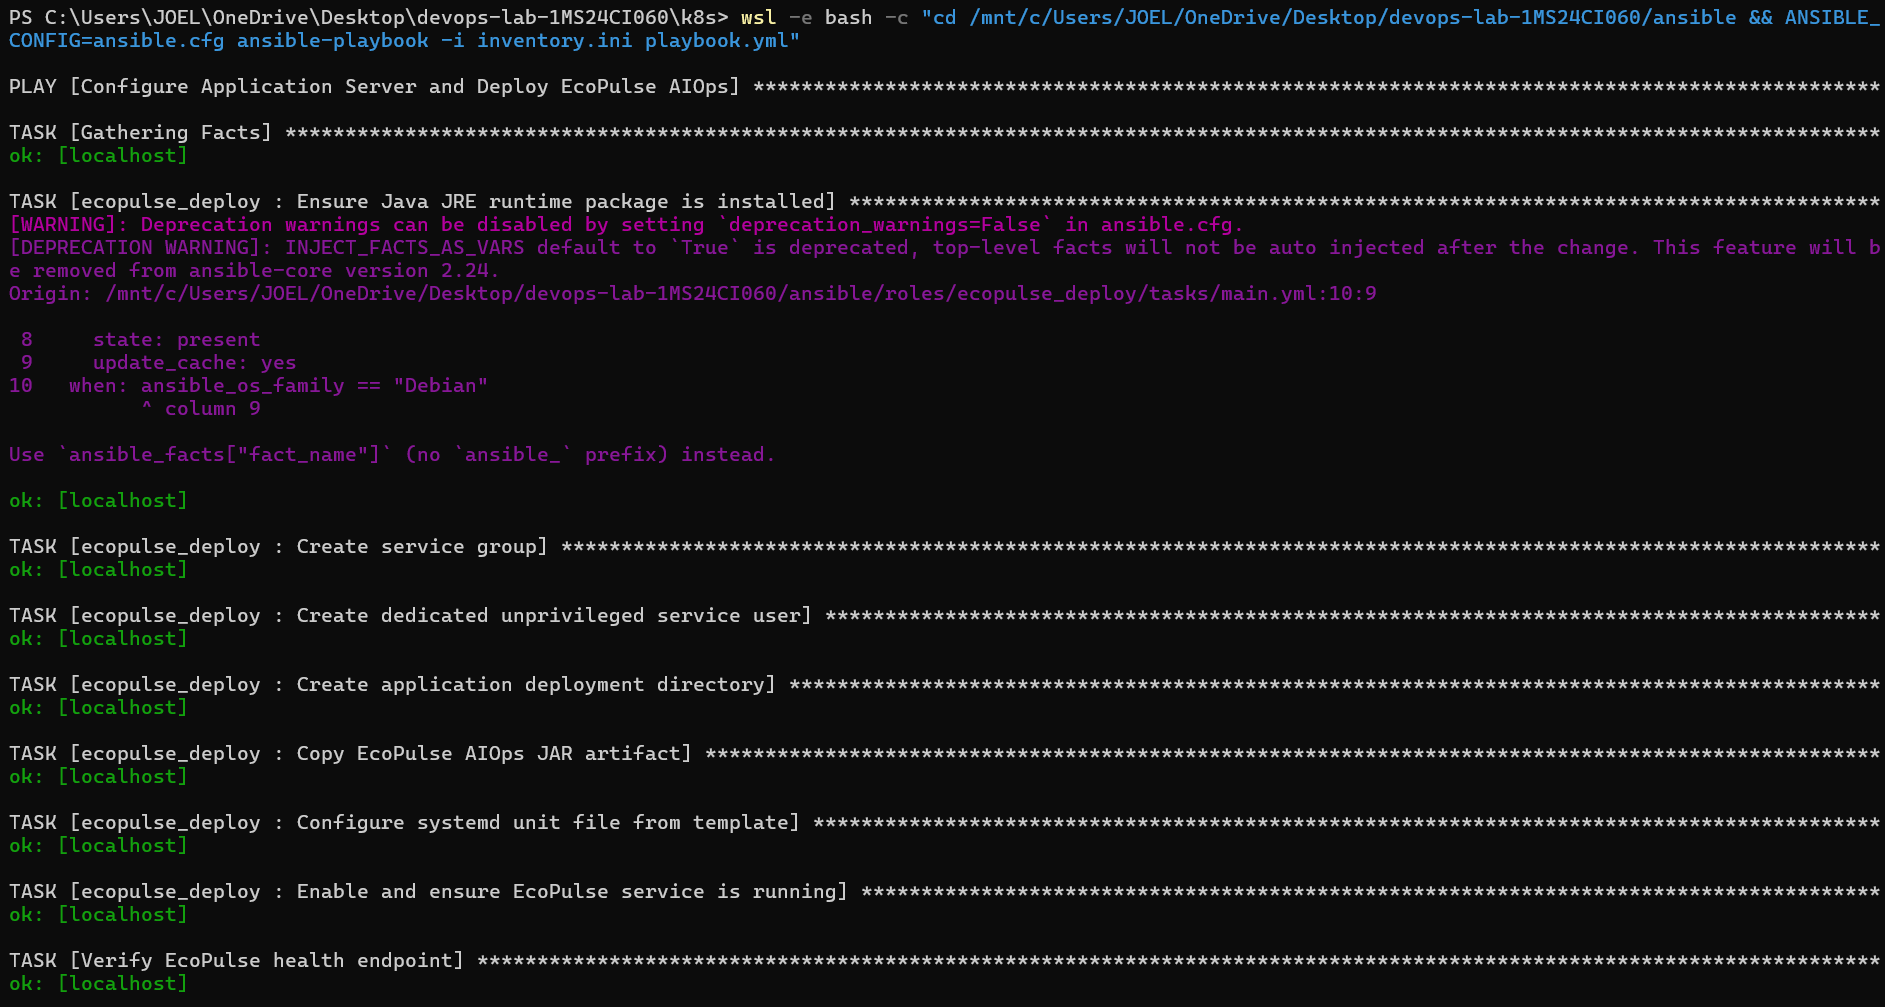
\includegraphics[width=0.90\linewidth]{screenshots/comp2_ansible_playbook.png}
    \caption{Ansible playbook execution displaying task execution across role and handlers.}
\end{figure}

\vspace{0.4cm}

\begin{figure}[H]
    \centering
    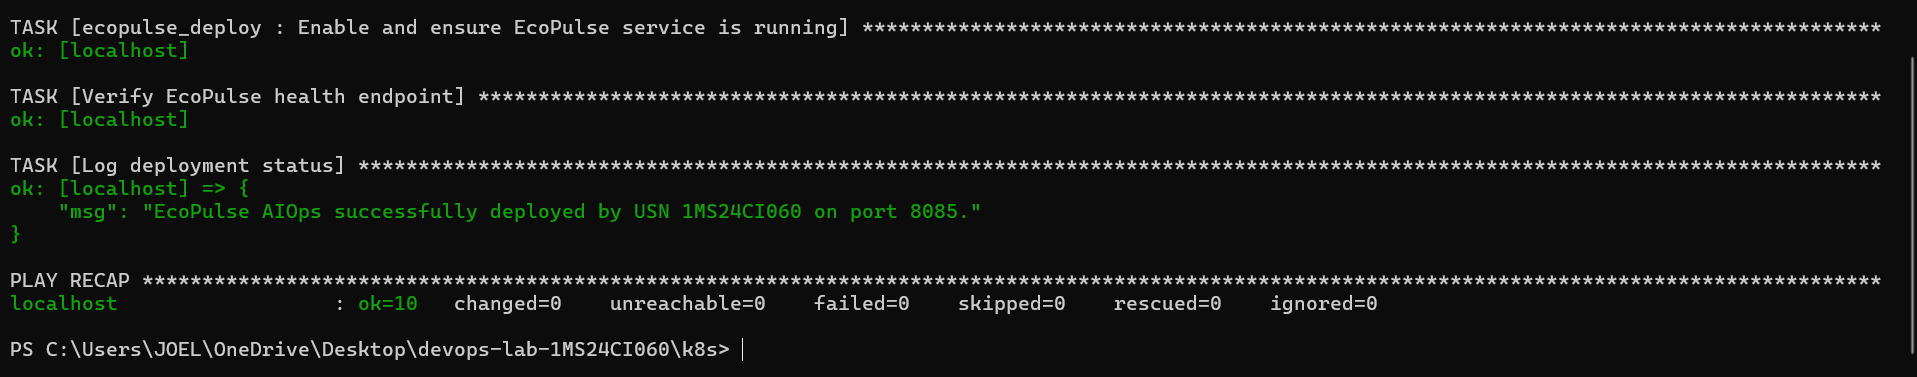
\includegraphics[width=0.90\linewidth]{screenshots/comp2_ansible_recap.png}
    \caption{Ansible PLAY RECAP verifying idempotency (\texttt{ok=10 changed=0 failed=0}) and USN logging.}
\end{figure}

\newpage

\begin{figure}[H]
    \centering
    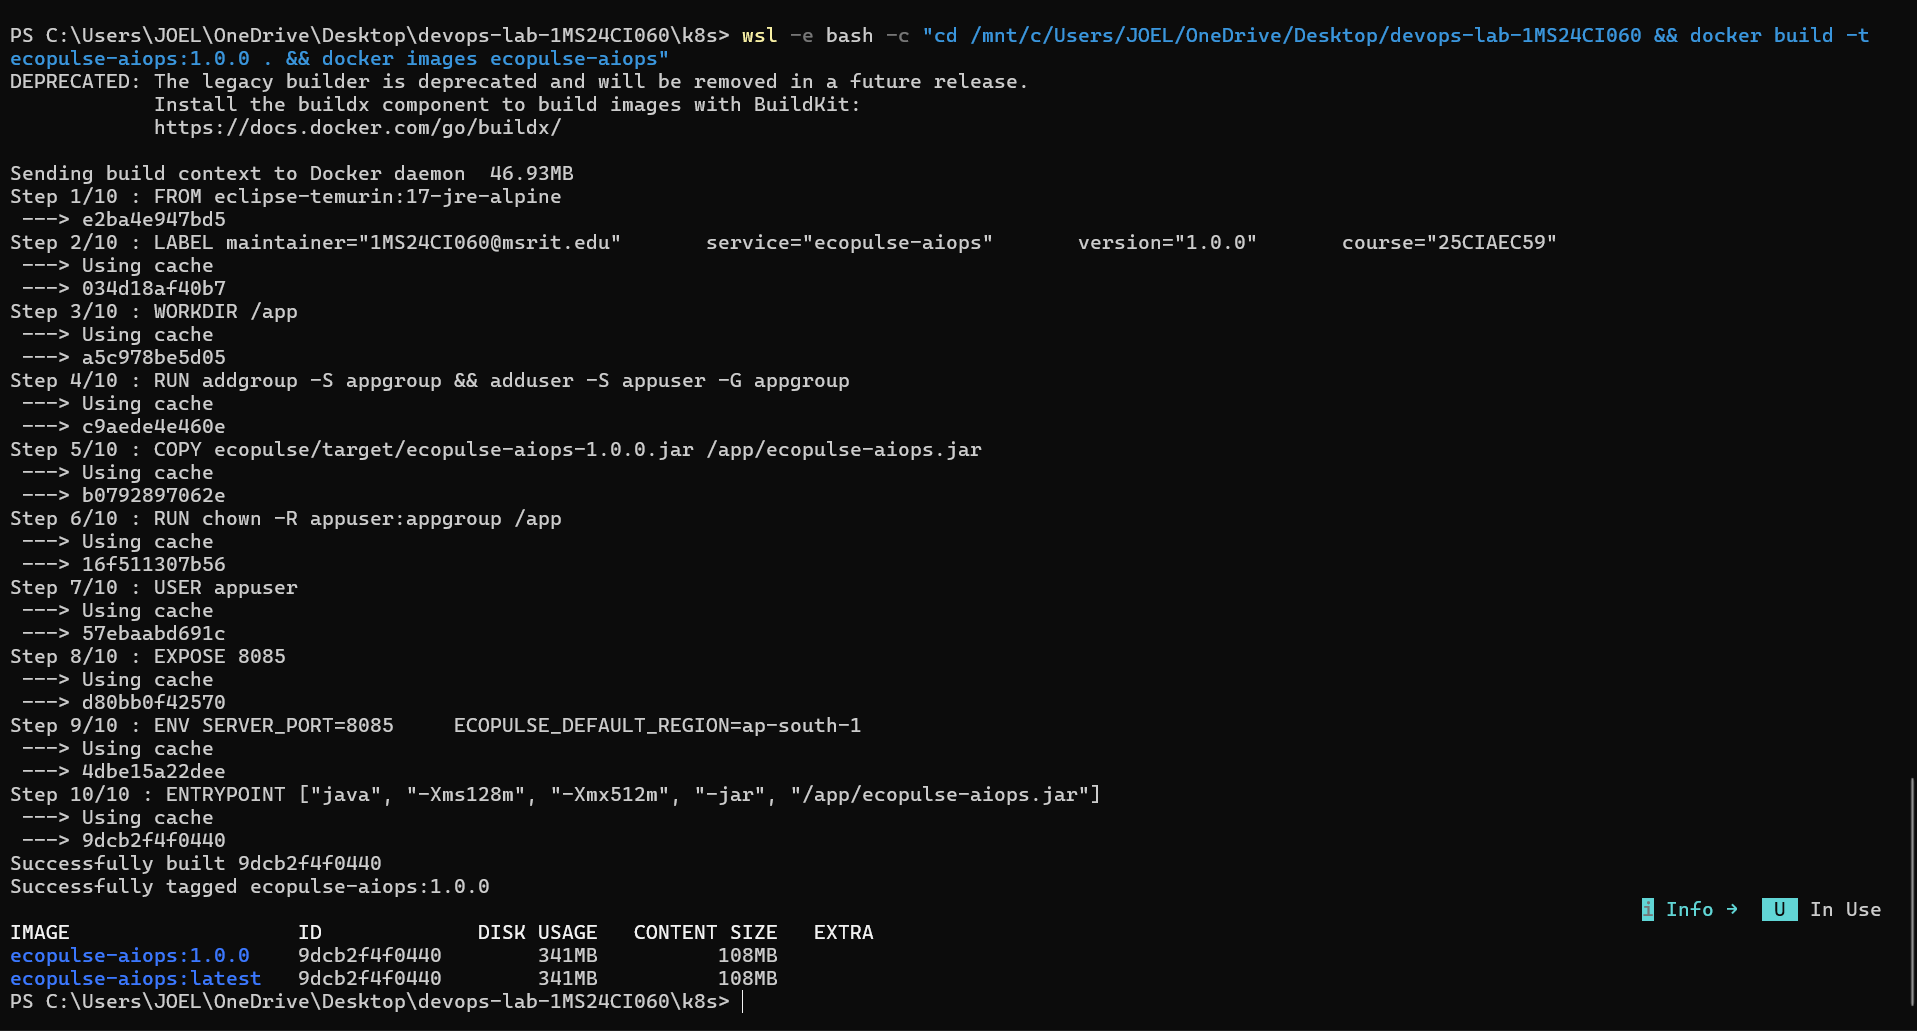
\includegraphics[width=0.90\linewidth]{screenshots/comp2_docker_build.png}
    \caption{Multi-stage Alpine Docker container build and image tagging for \texttt{ecopulse-aiops:1.0.0}.}
\end{figure}

\vspace{0.4cm}

\begin{figure}[H]
    \centering
    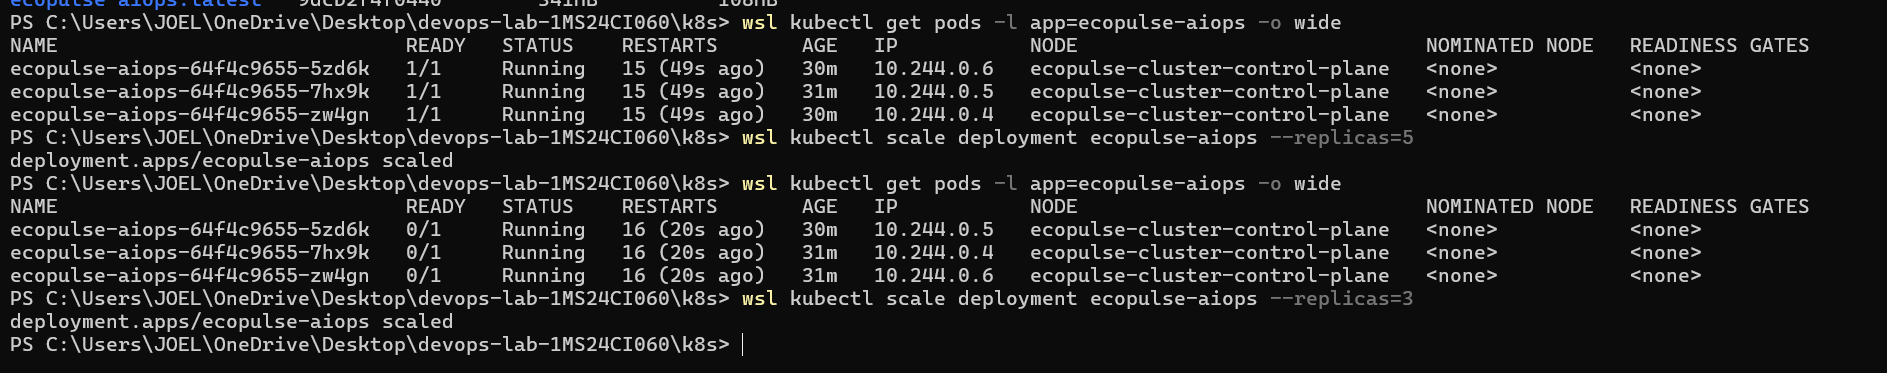
\includegraphics[width=0.90\linewidth]{screenshots/comp2_k8s_scaling.png}
    \caption{Kubernetes pod scaling from 3 to 5 replicas via \texttt{kubectl scale} command.}
\end{figure}

\newpage

\begin{figure}[H]
    \centering
    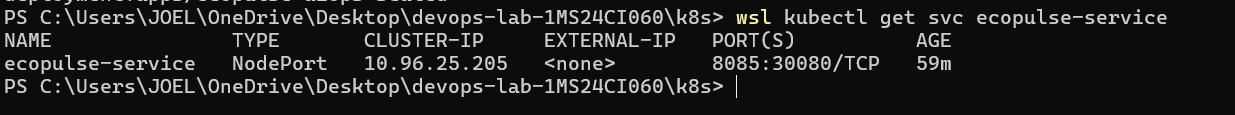
\includegraphics[width=0.90\linewidth]{screenshots/comp2_k8s_service.png}
    \caption{Kubernetes NodePort Service (\texttt{ecopulse-service}) routing port 8085 to node port 30080.}
\end{figure}

\vspace{0.4cm}

\begin{figure}[H]
    \centering
    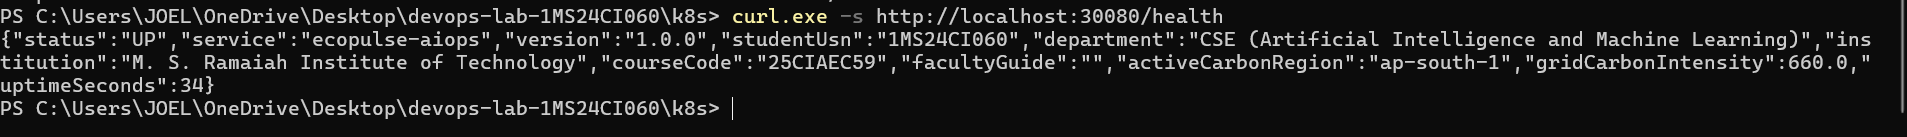
\includegraphics[width=0.90\linewidth]{screenshots/comp2_app_response.png}
    \caption{Terminal verification via curl showing live JSON telemetry response with USN \texttt{1MS24CI060}.}
\end{figure}

\newpage

\begin{figure}[H]
    \centering
    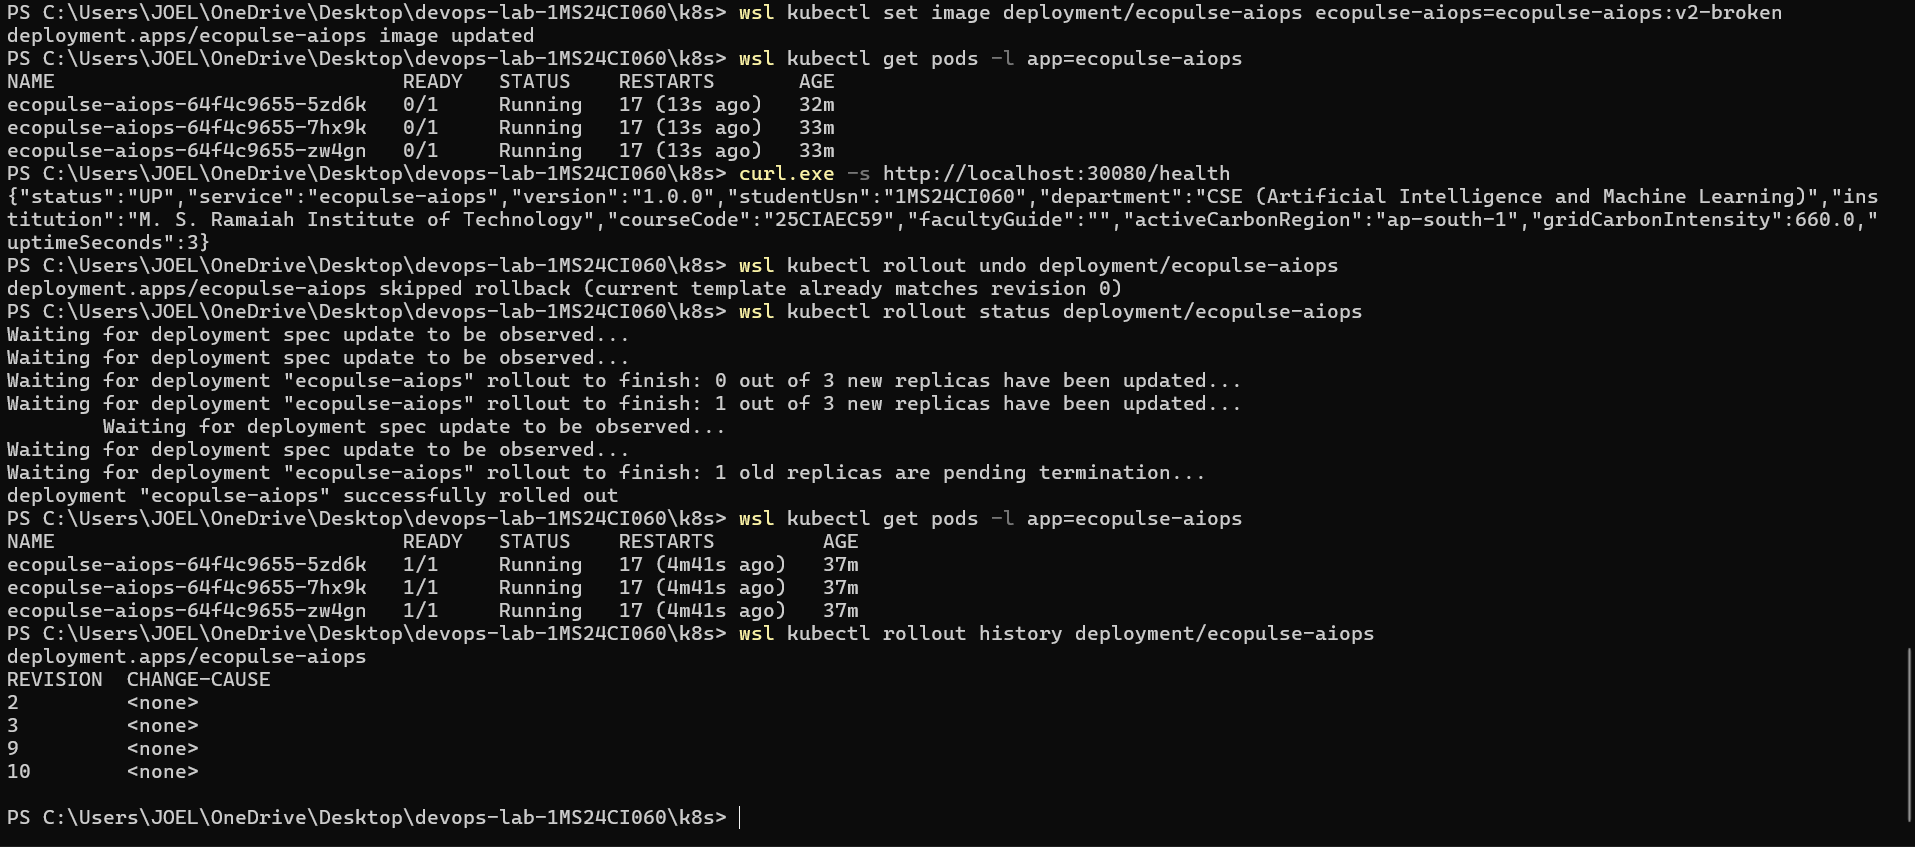
\includegraphics[width=0.90\linewidth]{screenshots/comp2_rollback_enhancement.png}
    \caption{Deployment Enhancement: Zero-downtime fault isolation during bad image rollout and recovery via \texttt{kubectl rollout undo}.}
\end{figure}

\vspace{0.4cm}

\begin{figure}[H]
    \centering
    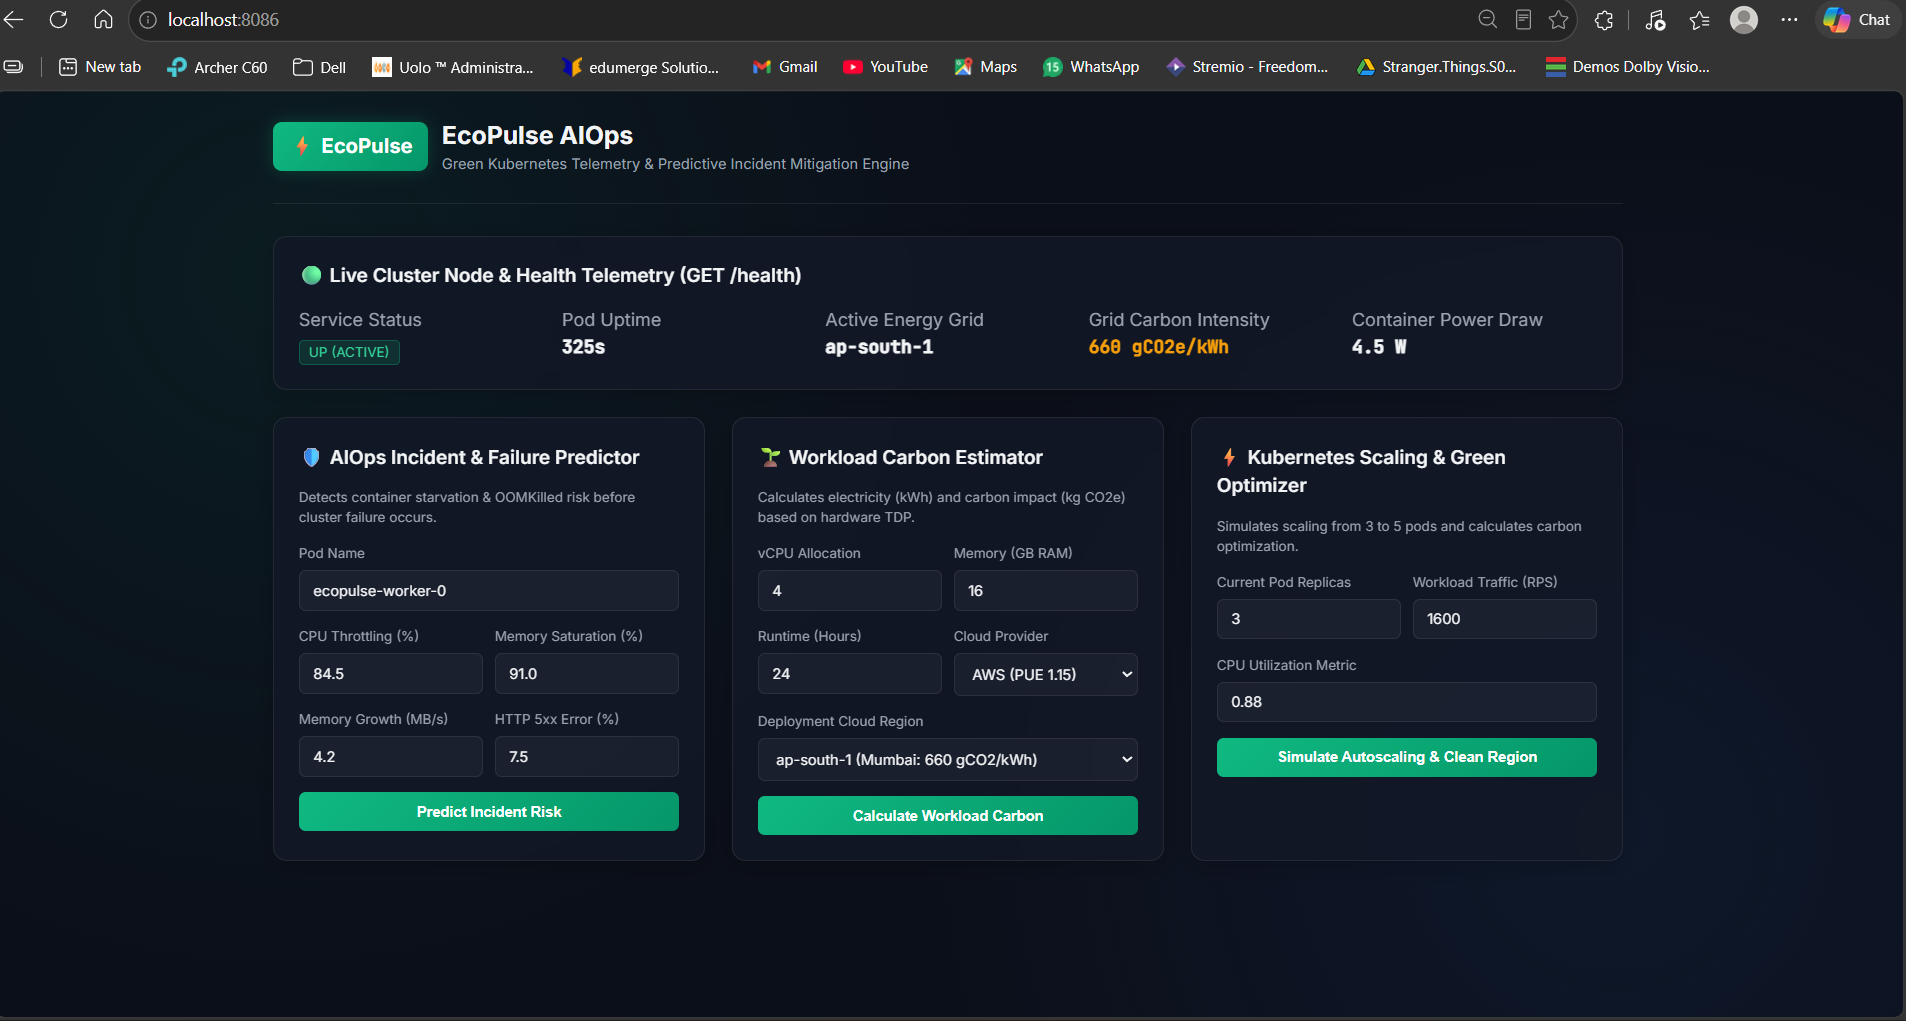
\includegraphics[width=0.90\linewidth]{screenshots/comp2_web_dashboard.png}
    \caption{Live interactive EcoPulse AIOps dashboard running on localhost displaying active cluster telemetry.}
\end{figure}

\subsection*{Conclusion}
Component 2 demonstrates the full deployment lifecycle. Ansible automates consistent system provisioning, while Docker provides lightweight, portable container runtimes. Kubernetes delivers robust cloud-native capabilities through self-healing, automated scaling, and rollback resilience, completing a production-grade DevOps assembly line.

\newpage

% ======================================================
% REFERENCES
% ======================================================
\section*{References}
\begin{enumerate}[nosep]
    \item Jennifer Davis and Katherine Daniels, \textit{Effective DevOps: Building a Culture of Collaboration, Affinity, and Tooling at Scale}, 1st Edition, O'Reilly Media, 2021.
    \item Sanjeev Sharma, \textit{The DevOps Adoption Playbook: A Guide to Adopting DevOps in a Multi-Speed IT Enterprise}, 1st Edition, Wiley, 2017.
    \item Official Git SCM Documentation -- \url{https://git-scm.com/doc}
    \item Official Jenkins CI Documentation -- \url{https://www.jenkins.io/doc/}
    \item Official Ansible Documentation -- \url{https://docs.ansible.com/}
    \item Official Kubernetes Documentation -- \url{https://kubernetes.io/docs/}
    \item Eclipse Temurin Container Images -- \url{https://hub.docker.com/_/eclipse-temurin}
    \item Spring Boot Reference Documentation (v3.2.5) -- \url{https://docs.spring.io/spring-boot/docs/3.2.5/reference/html/}
\end{enumerate}

\end{document}
